\documentclass[12pt]{article}
\usepackage[left=1cm, right=1cm, top=2cm,bottom=1.5cm]{geometry} 

\usepackage[parfill]{parskip}
\usepackage[utf8]{inputenc}
\usepackage[T2A]{fontenc}
\usepackage[russian]{babel}
\usepackage{enumitem}
\usepackage[normalem]{ulem}
\usepackage{amsfonts, amsmath, amsthm, amssymb, mathtools,xcolor,accents}
\usepackage{blkarray}

\usepackage{tabularx}
\usepackage{hhline}

\usepackage{accents}
\usepackage{fancyhdr}
\pagestyle{fancy}
\renewcommand{\headrulewidth}{1.5pt}
\renewcommand{\footrulewidth}{1pt}

\usepackage{graphicx}
\usepackage[figurename=Рис.]{caption}
\usepackage{subcaption}
\usepackage{float}

%%Наименование папки откуда забирать изображения
\graphicspath{ {./images/} }

%%Изменение формата для ввода доказательства
\renewcommand{\proofname}{$\square$  \nopunct}
\renewcommand\qedsymbol{$\blacksquare$}

%%Изменение отступа на таблицах
\addto\captionsrussian{%
	\renewcommand{\proofname}{$\square$ \nopunct}%
}
%% Римские цифры
\newcommand{\RN}[1]{%
	\textup{\uppercase\expandafter{\romannumeral#1}}%
}

%% Для удобства записи
\newcommand{\MR}{\mathbb{R}}
\newcommand{\MC}{\mathbb{C}}
\newcommand{\MQ}{\mathbb{Q}}
\newcommand{\MN}{\mathbb{N}}
\newcommand{\MZ}{\mathbb{Z}}
\newcommand{\MTB}{\mathbb{T}}
\newcommand{\MTI}{\mathbb{I}}
\newcommand{\MI}{\mathrm{I}}
\newcommand{\MCI}{\mathcal{I}}
\newcommand{\MCR}{\mathcal{R}}
\newcommand{\MJ}{\mathrm{J}}
\newcommand{\MH}{\mathrm{H}}
\newcommand{\MT}{\mathrm{T}}
\newcommand{\MU}{\mathcal{U}}
\newcommand{\MV}{\mathcal{V}}
\newcommand{\MA}{\mathcal{A}}
\newcommand{\MB}{\mathcal{B}}
\newcommand{\MF}{\mathcal{F}}
\newcommand{\ME}{\mathcal{E}}
\newcommand{\MW}{\mathcal{W}}
\newcommand{\ML}{\mathcal{L}}
\newcommand{\MM}{\mathcal{M}}
\newcommand{\MP}{\mathcal{P}}
\newcommand{\VN}{\varnothing}
\newcommand{\VE}{\varepsilon}
\newcommand{\dx}{\, dx}
\newcommand{\dy}{\, dy}
\newcommand{\dz}{\, dz}
\newcommand{\dd}{\, d}


\theoremstyle{definition}
\newtheorem{defn}{Опр:}
\newtheorem{rem}{Rm:}
\newtheorem{prop}{Утв.}
\newtheorem{exrc}{Упр.}
\newtheorem{problem}{Задача}
\newtheorem{lemma}{Лемма}
\newtheorem{theorem}{Теорема}
\newtheorem{corollary}{Следствие}

\newenvironment{cusdefn}[1]
{\renewcommand\thedefn{#1}\defn}
{\enddefn}

\DeclareRobustCommand{\divby}{%
	\mathrel{\text{\vbox{\baselineskip.65ex\lineskiplimit0pt\hbox{.}\hbox{.}\hbox{.}}}}%
}
\DeclareRobustCommand{\ndivby}{\mkern-1mu\not\mathrel{\mkern4.5mu\divby}\mkern1mu}


%Короткий минус
\DeclareMathSymbol{\SMN}{\mathbin}{AMSa}{"39}
%Длинная шапка
\newcommand{\overbar}[1]{\mkern 1.5mu\overline{\mkern-1.5mu#1\mkern-1.5mu}\mkern 1.5mu}
%Функция знака
\DeclareMathOperator{\sgn}{sgn}

%Функция ранга
\DeclareMathOperator{\rk}{\text{rk}}
\DeclareMathOperator{\diam}{\text{diam}}


%Обозначение константы
\DeclareMathOperator{\const}{\text{const}}

\DeclareMathOperator{\codim}{\text{codim}}

\DeclareMathOperator*{\dsum}{\displaystyle\sum}
\newcommand{\ddsum}[2]{\displaystyle\sum\limits_{#1}^{#2}}
\newcommand{\ddssum}[2]{\displaystyle\smashoperator{\sum\limits_{#1}^{#2}}}
\newcommand{\ddlsum}[2]{\displaystyle\smashoperator[l]{\sum\limits_{#1}^{#2}}}
\newcommand{\ddrsum}[2]{\displaystyle\smashoperator[r]{\sum\limits_{#1}^{#2}}}

%Интеграл в большом формате
\DeclareMathOperator{\dint}{\displaystyle\int}
\newcommand{\ddint}[2]{\displaystyle\int\limits_{#1}^{#2}}
\newcommand{\ssum}[1]{\displaystyle \sum\limits_{n=1}^{\infty}{#1}_n}

\newcommand{\smallerrel}[1]{\mathrel{\mathpalette\smallerrelaux{#1}}}
\newcommand{\smallerrelaux}[2]{\raisebox{.1ex}{\scalebox{.75}{$#1#2$}}}

\newcommand{\smallin}{\smallerrel{\in}}
\newcommand{\smallnotin}{\smallerrel{\notin}}

\newcommand*{\medcap}{\mathbin{\scalebox{1.25}{\ensuremath{\cap}}}}%
\newcommand*{\medcup}{\mathbin{\scalebox{1.25}{\ensuremath{\cup}}}}%

\makeatletter
\newcommand{\vast}{\bBigg@{3.5}}
\newcommand{\Vast}{\bBigg@{5}}
\makeatother

%Промежуточное значение для sup\inf, поскольку они имеют разную высоту
\newcommand{\newsup}{\mathop{\smash{\mathrm{sup}}}}
\newcommand{\newinf}{\mathop{\mathrm{inf}\vphantom{\mathrm{sup}}}}

%Скалярное произведение
\newcommand{\inner}[2]{\left\langle #1, #2 \right\rangle }
\newcommand{\linsp}[1]{\left\langle #1 \right\rangle }
\newcommand{\linmer}[2]{\left\langle #1 \vert #2\right\rangle }

%Подпись символов снизу
\newcommand{\ubar}[1]{\underaccent{\bar}{#1}}

%%Шапка для букв сверху
\newcommand{\wte}[1]{\widetilde{#1}}
\newcommand{\wht}[1]{\widehat{#1}}
\newcommand{\ovl}[1]{\overline{#1}}


%%Трансформация Фурье
\newcommand{\fourt}[1]{\mathcal{F}\left(#1\right)}
\newcommand{\ifourt}[1]{\mathcal{F}^{-1}\left(#1\right)}

%%Символ вектора
\newcommand{\vecm}[1]{\overrightarrow{#1\,}}

%%Пространстов матриц
\newcommand{\matsq}[1]{\operatorname{Mat}_{#1}}
\newcommand{\mat}[2]{\operatorname{Mat}_{#1, #2}}

%Оператор для действ и мнимых чисел
\DeclareMathOperator{\IM}{\operatorname{Im}}
\DeclareMathOperator{\RE}{\operatorname{Re}}
\DeclareMathOperator{\li}{\operatorname{li}}
\DeclareMathOperator{\GL}{\operatorname{GL}}
\DeclareMathOperator{\SL}{\operatorname{SL}}
\DeclareMathOperator{\Char}{\operatorname{char}}
\DeclareMathOperator\Arg{Arg}
\DeclareMathOperator\ord{ord}

%Оператор для образа
\DeclareMathOperator{\Ima}{Im}

%Делимость чисел
\newcommand{\modn}[3]{#1 \equiv #2 \; (\bmod \; #3)}
\newcommand{\nmodn}[3]{#1 \not\equiv #2 \; (\bmod \; #3)}

%%Взятие в скобки, модули и норму
\newcommand{\parfit}[1]{\left( #1 \right)}
\newcommand{\modfit}[1]{\left| #1 \right|}
\newcommand{\sqparfit}[1]{\left\{ #1 \right\}}
\newcommand{\normfit}[1]{\left\| #1 \right\|}

%%Функция для обозначения равномерной сходимости по множеству
\newcommand{\uconv}[1]{\overset{#1}{\rightrightarrows}}
\newcommand{\uconvm}[2]{\overset{#1}{\underset{#2}{\rightrightarrows}}}

%% Функция для добавления круга сверху множества
\newcommand{\Circ}[1]{\accentset{\circ}{#1}}

%%Функция для обозначения нижнего и верхнего интегралов
\def\upint{\mathchoice%
	{\mkern13mu\overline{\vphantom{\intop}\mkern7mu}\mkern-20mu}%
	{\mkern7mu\overline{\vphantom{\intop}\mkern7mu}\mkern-14mu}%
	{\mkern7mu\overline{\vphantom{\intop}\mkern7mu}\mkern-14mu}%
	{\mkern7mu\overline{\vphantom{\intop}\mkern7mu}\mkern-14mu}%
	\int}
\def\lowint{\mkern3mu\underline{\vphantom{\intop}\mkern7mu}\mkern-10mu\int}

%%След матрицы
\DeclareMathOperator*{\tr}{tr}

\DeclareMathOperator*{\symdif}{\bigtriangleup}

\makeatletter
\renewcommand*\env@matrix[1][*\c@MaxMatrixCols c]{%
	\hskip -\arraycolsep
	\let\@ifnextchar\new@ifnextchar
	\array{#1}}
\makeatother


%% Переопределение функции хи, чтобы выглядела более приятно
\makeatletter
\@ifdefinable\@latex@chi{\let\@latex@chi\chi}
\renewcommand*\chi{{\@latex@chi\smash[t]{\mathstrut}}} % want only bottom half of \mathstrut
\makeatletter

\setcounter{MaxMatrixCols}{20}

\begin{document}
\lhead{Действительный анализ}
\chead{Дьяченко М.И.}
\rhead{Лекция - 5}

\section*{Неизмеримые множества}

Хотелось бы понять какие существуют неизмеримые множества и насколько может быть богатой Лебеговская $\sigma$-алгбера. На самом деле, ответ на вопрос существуют ли такие множества относительно любой меры зависит, в общем, от двух вещей: самой меры и принятия или нет аксиомы выбора. В данном курсе мы принимаем аксиому выбора безоговорочно $\Rightarrow$ всё зависит от меры.

Пусть $M$ это все подмножества прямой $\MR^1$ и мера задана следующим образом:
$$
	\mu(A) = 
	\begin{cases}
		1, & 0 \in A \\
		0, & 0 \not\in A 
	\end{cases}
$$ 
Несложно понять, что это мера Лебега-Стильтьеса, порожденная функцией: $\varphi(x) = \MTI(x > 0)$, то есть она непрерывна слева. В этом случае неизмеримых множеств нет. В более привычном случае классической меры Лебега, с принятой аксиомой выбора, неизмеримых множеств будет достаточно. Основное свойство, которое их порождает это инвариантность классической меры, относительно сдвига.

\begin{theorem}
	Пусть $\MM$ это классическая Лебеговская $\sigma$-алгебра на подмножествах отрезка $[0,1]$, $\mu$ - соответствующая классическая мера Лебега, $A \in \MM$ и $\mu(A) > 0$. Тогда:
	$$
		\exists \, B \subset A \colon B \not\in \MM
	$$
\end{theorem}
\begin{rem}
	Иными словами, в любом множестве положительной меры (относительно классической меры Лебега) есть неизмеримое подмножество. Также заметим, что условие $\mu(A) > 0$ существенно, поскольку мы знаем, что мера Лебега полна и поэтому если имеем множество меры нуль, то автоматически любое его подмножество будет измеримо и тоже будет иметь нулевую меру, тогда как в множествах положительной меры будут неизмеримые подмножества.
\end{rem}
\begin{proof}
	Введём на $[0,1]$ отношение эквивалентности: $x \sim y \Leftrightarrow x - y \in \MQ$. Рефлексивность, симметричность и транзитивность - очевидны. Тогда $[0,1]$ может быть представлен следующим образом: 
	$$
		[0,1] = \bigsqcup\limits_{\alpha \in \Omega}K_\alpha
	$$
	где $K_\alpha$ - классы (утверждение доказывается в других курсах или см. Кострикина), а объединение не является счетным. Используя аксиому выбора, образуем множество: 
	$$
		E_0 = \{x_\alpha\}_{\alpha \in \Omega}, \, x_\alpha \in K_\alpha, \, \forall \alpha \in \Omega
	$$ 
	Затем, пусть $\{r_n\}_{n = 0}^{\infty} = \MQ \cap [-1,1]$, где для удобства будем считать, что $r_0 = 0$. Обозначим, через $E_n = E_0 + r_n = \{x_\alpha + r_n, \, \alpha \in \Omega\}, \, n \in \MN, n > 0$. Докажем, ряд утверждений:
	\begin{enumerate}[label = \arabic*)]
		\item $E_n \cap E_m = \VN$ при $n \neq m$; 
		\begin{proof}
			Действительно, пусть существует общий элемент $z$:
			$$
				\exists \, z \in E_n \cap E_m \Rightarrow x_\alpha + r_n  = z = x_\beta + r_m \Rightarrow x_\alpha - x_\beta = r_n - r_m \in \MQ \Rightarrow 
			$$
			$$
				\Rightarrow x_\alpha \sim x_\beta \Rightarrow \alpha = \beta, \, x_\alpha = x_\beta \Rightarrow r_n = r_m \Rightarrow n = m
			$$
			где равенства представителей классов верны, поскольку из каждого класса мы взяли по одному представителю;
		\end{proof}
		\item $[0,1] \subset \bigsqcup\limits_{n = 0 }^{\infty}E_n$;
		\begin{proof}
			Пусть $x \in [0,1]$, тогда в силу представления $[0,1]$ верно: 
			$$
				\exists \, \alpha_0 \colon x \in K_{\alpha_0} \Rightarrow x - x_{\alpha_0} = q  \in [-1,1] \wedge q \in \MQ \Rightarrow q = r_{n_0} \Rightarrow x = x_{\alpha_0} + r_{n_0} \in E_{n_0}
			$$
			Таким образом, $\forall x \in [0,1], \, \exists \, E_k \colon x \in E_k \Rightarrow [0,1] \subset \bigsqcup\limits_{n = 0 }^{\infty}E_n$;
		\end{proof}
	\end{enumerate}
	Поскольку $[0,1] \subset \bigsqcup\limits_{n = 0 }^{\infty}E_n$ и так как $A \subset [0,1]$, то будет верно: 
	$$
		A = \bigsqcup\limits_{n = 0 }^{\infty}(A \cap E_n) = \bigsqcup\limits_{n = 0 }^{\infty}A_n, \, \forall n, \, A_n = A \cap E_n
	$$
	Предположим, что $\forall n, \, A_n \in \MM$, то есть измеримое множество $\Rightarrow$ в силу $\sigma$-аддитивности классической меры Лебега будет верно:
	$$
		\mu(A) = \ddsum{n = 0}{\infty}\mu(A_n), \, \mu(A) > 0 \Rightarrow \exists \, n_s \colon \mu(A_{n_s}) = \gamma > 0
	$$
	По определению, $A_{n_s} \subset E_{n_s}$. Рассмотрим при $n \neq n_s$ множества: $C_n = A_{n_s} - r_{n_s} + r_n \subset E_n$, поскольку:
	$$
		A_{n_s} \subset E_{n_s} \Rightarrow A_{n_s} - r_{n_s} \subset E_0 \Rightarrow A_{n_s} - r_{n_s} + r_n \subset E_n
	$$
	Также, положим: $C_{n_s} = A_{n_s}$. Так как классическая мера Лебега инвариантна относительно сдвигов (см. лекция $3$, после следствия $2$), то $\forall n,\, C_n \in \MM$ - тоже измеримое множество, поскольку $A_{n_s} \in \MM$ и мера равна: $\forall n, \, \mu(C_n) = \gamma$. Поэтому:
	$$
		\forall n,\, C_n \subset E_n  \wedge \forall n \neq m, \, E_n \cap E_m = \VN \Rightarrow C_n \cap C_m = \VN \Rightarrow \bigsqcup\limits_{n = 0}^{\infty}C_n \subseteq \bigsqcup\limits_{n = 0}^{\infty} E_n \subseteq [-1,2]
	$$
	где последнее следует из определения $E_0 \subset [0,1]$ и того, что $r_n \in [-1,1]$. Тогда:
	$$
		\infty = \ddsum{n = 0}{\infty}\gamma = \ddsum{n = 0}{\infty} \mu(C_n)  \leq \mu([-1,2]) = 2 - (-1) = 3
	$$
	Получили противоречие с тем, что: $A_n = A \cap E \in \MM$, то есть это измеримые множества. В результате:
	$$
		\exists \, n_1 \colon A_{n_1} = A \cap E_{n_1} \not\in \MM 
	$$
	Следовательно, $B = A_{n_1}$ это неизмеримое множество, существование которого мы хотели доказать.
\end{proof}

\newpage
\section*{Некоторые свойства измеримых множеств}
Сначала разберем техническую теорему, которая пригодится при разборе теоремы Фубини.
\begin{theorem}
	Пусть $\MM$ - $\sigma$-алгебра на которой задана $\sigma$-аддитивная, $\sigma$-конечная мера Лебега $\mu$, полученная Лебеговским продолжением $\sigma$-аддитивной меры $m$ с полукольца $S$. Пусть $A \in \MM$ и $\mu(A) < \infty$. Тогда $A$ можно представить в виде:
	$$
		A = \bigcap\limits_{i = 1}^{\infty}\bigcup\limits_{j = 1}^{\infty}A_{i,j} \setminus A_0, \; A_{i,j} \in \MCR(S), \; A_0 \in \MM, \, \mu(A_0) = 0
	$$
	где $\MCR(S)$ это минимальное кольцо, содержащее $S$. Для каждого фиксированного $i$ выполняется вложение множеств: $\forall i, \, A_{i,1} \subseteq A_{i,2} \subseteq \dotsc$. Если $B_{i} = \bigcup\limits_{j = 1}^{\infty}A_{i,j}$, то $\mu(B_1) < \infty$ и $B_1 \supseteq B_2 \supseteq \dotsc$.
\end{theorem}
\begin{proof}
	Из процесса построения конечной и $\sigma$-конечной меры Лебега следует, что: $\forall n, \, \exists \, \{C_{n,i}\}_{i=1}^{\infty} \subset S$ такое, что выполняются следующие условия: 
	$$
		A \subset \bigcup\limits_{i = 1}^{\infty}C_{n,i}, \quad \mu\left(\bigcup\limits_{i = 1}^{\infty}C_{n,i} \setminus A\right) < \dfrac{1}{n}
	$$ 
	Это можно получить сразу из определения меры Лебега, поскольку $\mu(A)$ это точная нижняя грань: 
	$$
		\forall n, \, \exists \, \{C_{n,i}\}_{i=1}^{\infty} \subset S \colon \mu\left(\bigcup\limits_{i = 1}^{\infty}C_{n,i} \right) \leq \mu(A) + \dfrac{1}{n}, \, S \subseteq \MM \Rightarrow  \bigcup\limits_{i = 1}^{\infty}C_{n,i} \in \MM \Rightarrow
	$$
	$$
		\Rightarrow 0 < \mu\left(\bigcup\limits_{i = 1}^{\infty}C_{n,i} \setminus A\right) = \mu\left(\bigcup\limits_{i = 1}^{\infty}C_{n,i} \right) - \mu(A) \leq \dfrac{1}{n}
	$$
	где $A = B \sqcup (A \setminus B) \Rightarrow \mu(A) = \mu(A \setminus B) + \mu(B)$ верно для $A,B \in \MM$ (измеримых по Лебегу множеств, где $\mu$ является мерой). Предположим: 
	$$
		B_1 = \bigcup\limits_{l = 1}^{\infty}C_{1,l}, \, \forall i > 1, \, B_i = \bigcap\limits_{k = 1}^{i}\bigcup\limits_{l = 1}^{\infty}C_{k,l}
	$$ 
	Тогда очевидно:
	$$
		\mu(B_1) = \mu\left(\bigcup\limits_{l = 1}^{\infty}C_{1,l}\right) \leq \mu(A) + \dfrac{1}{n} < \infty
	$$
	Затем, по определению, мы получаем: $B_1 \supseteq B_2 \supseteq \dotsc$, поскольку множества $C_{k,l}$ пересекаются в определении $B_i$. Кроме того, $\forall i, \, B_i \supseteq A$, из условий выше. Перегруппируем слагаемые в $B_i$:
	$$
		\forall i, \, B_i = \bigcap\limits_{k = 1}^{i}\bigcup\limits_{l = 1}^{\infty}C_{k,l} =  \bigcup\limits_{l_1 = 1}^{\infty}\bigcup\limits_{l_2 = 1}^{\infty}\dotsc\bigcup\limits_{l_i = 1}^{\infty}(C_{1,l_1}\cap C_{2,l_2} \cap \dotsc \cap C_{i,l_i})
	$$
	Поскольку $C_{1,l_1}\cap C_{2,l_2} \cap \dotsc \cap C_{i,l_i}$ это конечное пересечение элементов полукольца, то это слагаемое принадлежит $S$, в результате счётное объединение таких слагаемых можно переписать:
	$$
		\forall i, \, B_i = \bigcup\limits_{l_1 = 1}^{\infty}\bigcup\limits_{l_2 = 1}^{\infty}\dotsc\bigcup\limits_{l_i = 1}^{\infty}(C_{1,l_1}\cap C_{2,l_2} \cap \dotsc \cap C_{i,l_i}) = \bigcup\limits_{r = 1}^{\infty}D_{i,r}, \, D_{i,r} \in S
	$$
	Тогда положим при $j \geq 1$ множество: 
	$$
		\forall j \geq 1, \, A_{i,j} = \bigcup\limits_{r = 1}^{j}D_{i,r} \in \MCR(S) \Rightarrow \forall i, \, B_i = \bigcup\limits_{r = 1}^{\infty}D_{i,r} = \bigcup\limits_{j = 1}^{\infty}\bigcup\limits_{r = 1}^{j}D_{i,r} = \bigcup\limits_{j = 1}^{\infty}A_{i,j}
	$$ 
	где $A_{i,j} \in \MCR(S)$ поскольку $\MCR(S)$ это кольцо и выдерживает конечное объединение. При этом верна вложенность: $\forall i, \, A_{i,1} \subseteq A_{i,2} \subseteq \dotsc$  просто по определению. Определим множество $A_0$:
	$$
		A_0 = \bigcap\limits_{i = 1}^{\infty}B_i \setminus A \Rightarrow \forall i, \, A_0 \subseteq B_i, \, \mu(B_i \setminus A) \leq \mu\left(\bigcup\limits_{l = 1}^{\infty}C_{i,l} \setminus A\right) < \dfrac{1}{i} \Rightarrow \forall i, \, \mu(A_0) < \dfrac{1}{i}
	$$
	так как $B_i$ это пересечение объединений из $C_{i,l}$, тогда $A_0 \in \MM$ (вытекает из $\sigma$-алгебры: она выдерживает все операции) и $\mu(A_0) = 0$ в силу произвольности $i$. Итого:
	$$
		\forall i, \, A \subseteq B_i \Rightarrow A \subseteq \bigcap\limits_{i = 1}^{\infty}B_i \Rightarrow \bigcap\limits_{i = 1}^{\infty}\bigcup\limits_{j = 1}^{\infty}A_{i,j} \setminus A_0 = \bigcap\limits_{i = 1}^{\infty}B_i \setminus \left(\bigcap\limits_{i = 1}^{\infty}B_i \setminus A \right) = A \cap \bigcap\limits_{i = 1}^{\infty}B_i = A
	$$
	где предпоследнее равенство верно в силу:
	$$	
		x \in A \cap B \Leftrightarrow x \in A \wedge x \in B \Leftrightarrow x \in A \wedge x \not\in A\setminus B \Leftrightarrow x \in A \setminus (A \setminus B)
	$$
\end{proof}

\begin{rem}
	Из этого же результата, когда речь идет про классическую меру Лебега на отрезке $[0,1]$, можно вывести что любое измеримое множество может быть представлено либо в виде пересечения счётного числа открытых множеств минус множество меры нуль, либо в виде объединения счётного числа замкнутых множеств плюм множество меры нуль. То есть либо множество типа $G_\delta$ без множества меры нуль, либо множество типа $F_\sigma$ которому добавили множество меры нуль.
\end{rem}

\begin{defn}
	Пусть $E \subset \MR^1$ и $K$ - система невырожденных отрезков ($[a,b]$ - невырожден $\Leftrightarrow b > a$). Тогда говорят, что $E$ \uwave{покрыто системой} $K$ \uwave{в смысле Витали} в том и только в том случае, когда:
	$$
		\forall x \in E, \, \forall \VE > 0, \, \exists \, \text{ отрезок } \MI = \MI_{x,\VE} \in K \colon x \in \MI \wedge \mu(\MI) < \VE
	$$
	где $\mu$ - классическая мера Лебега (длина).
\end{defn}

\begin{theorem}(\textbf{Витали})
	Пусть ограниченное множество $E$ лежит на прямой $E \subset \MR^1$ и система невырожденных отрезков $K$ покрывает $E$ в смысле Витали. Тогда $\exists$ система попарно непересекающихся отрезков $\{\MI_n\}_{n = 1}^{\infty} \subset K$ такая, что:
	$$
		\mu^*\left(E \setminus \bigsqcup\limits_{n = 1}^{\infty}\MI_n\right) = 0
	$$
	где $\mu^*$ это классическая внешняя мера Лебега.
\end{theorem}
\begin{proof}
	Пусть $E \subseteq [a,b]$, так как $E$ по условию ограниченно. Поскольку система $K$ покрывала $E$ в смысле Витали, то система: 
	$$
		K_1 = \{\MI \in K \colon \MI \subseteq [a-1,b+1]\}
	$$ 
	также покрывает $E$ в смысле Витали. Определим число: 
	$$
		\alpha_1 = \sup\limits_{\MI \in K_1}\mu(\MI)
	$$ 
	где $\alpha_1 > 0$ в силу того, что мы не рассматриваем невырожденные отрезки. Поскольку в $K_1$ все $\MI$ лежат в конечном отрезке, то $\alpha_1 < \infty$ и можно выбрать $\MI_1 \in K_1 \colon \mu(\MI_1) > \tfrac{\alpha_1}{2}$. Определим множество: 
	$$
		K_2 = \{\MI \in K_1 \colon \MI \cap \MI_1 = \VN\}
	$$ 
	Если $K_2 = \VN$, то заканчиваем процесс, в противном случае, полагаем:
	$$
		\alpha_2 = \sup\limits_{\MI \in K_2}\mu(\MI) \Rightarrow \exists \, \MI_2 \in K_2 \colon \mu(\MI_2) > \dfrac{\alpha_2}{2}
	$$ 
	И так далее, возможны два случая:
	\begin{enumerate}[label=\arabic*)]
		\item $\exists \, n_0 \colon K_{n_0} = \VN$, то есть процесс на каком-то шаге обрывается. Тогда мы имеем систему попарно непересекающихся отрезков: $\MI_1, \dotsc, \MI_{n_0 -1} \subset K$. Предположим, что: 
		$$
			\exists \, x \colon x \in E \setminus \bigsqcup\limits_{l = 1}^{n_0 - 1}\MI_l = E \setminus F, \, F = \bigsqcup\limits_{l = 1}^{n_0 - 1}\MI_l
		$$
		конечное объединение замкнутых множеств - замкнуто $\Rightarrow F$ - замкнутое множество. Тогда: 
		$$
			\rho(x,F) = \inf\limits_{y \in F} |x -y| = \alpha > 0
		$$
		но по условию $\exists$ отрезок $\MI_{x,\alpha/2} \in K_1 \colon x \in \MI_{x,\alpha/2} \wedge \mu(\MI_{x,\alpha/2}) < \tfrac{\alpha}{2}$, тогда: $\MI_{x,\alpha/2} \cap F = \VN$, поскольку если бы было непустое пересечение, то расстояние: 
		$$
			\alpha = \rho(x,F) < \dfrac{\alpha}{2}
		$$
		получили противоречие с утверждением, что $K_{n_0} = \VN$, поскольку нашли отрезок который подходит на роль отрезка из $K_{n_0}$. Таким образом, $E \subset F$ и утверждение  доказано. Мера будет равна $0$ потому, что $E \subset F = \VN$;
		\item Построена счётная система попарно непересекающихся отрезков $\{\MI_n\}_{n = 1}^{\infty} \subset K_1$, причем: 
		$$
			\forall n, \, \mu(\MI_n) > \dfrac{\alpha_n}{2}, \, \alpha_n = \sup\limits_{\MI \in K_n} \mu(\MI)
		$$
		Возьмем некоторое число $\gamma > 0$, тогда так как $\bigsqcup\limits_{n = 1}^{\infty}\MI_n \subseteq [a- 1, b+ 1]$, то будет верно:
		$$
			\ddsum{n = 1}{\infty}\mu(\MI_n) < \infty \Rightarrow \exists \, N = N(\gamma) \colon \ddsum{n = N}{\infty}\mu(\MI_n) < \dfrac{\gamma}{5}
		$$
		$$
			x \in E \setminus \bigsqcup\limits_{n = 1}^{\infty}\MI_n  \Rightarrow  x \in E \setminus \bigsqcup\limits_{n = 1}^{N}\MI_n , \, F_N = \bigsqcup\limits_{n = 1}^{N}\MI_n \Rightarrow \rho(x, F_N)  > 0
		$$ 
		поэтому $\exists \, \MI_x \in K_{N+1}$ - отрезок из $K_1 \colon x \in \MI_x \wedge \MI_x \cap F_N = \VN$ (проверяли в предыдущем пункте). Очевидно, что: 
		$$
			\lim\limits_{n\to \infty}\alpha_n  = 0
		$$ 
		причем, стремится монотонно, поскольку уменьшается множество по которому берется точная верхняя грань, сам же предел верен, в силу следующего:
		$$
			\forall n, \, \mu(\MI_n) > \dfrac{\alpha_n}{2}, \, \alpha_n = \sup\limits_{\MI \in K_n} \mu(\MI) \wedge \MI_n \in K_1 \Rightarrow \mu(\MI_n) \leq \mu([a-1,b+1]) = b - a + 2 < \infty
		$$
		все отрезки лежат на конечном отрезке и туда нельзя вложить бесконечно много отрезков меры больше какого-то числа. Поэтому: 
		$$
			\exists \, l > N + 1 \colon \MI_x \not\in K_l \Rightarrow \exists \, m \geq N+ 1 \colon \MI_x \in K_m \setminus K_{m + 1}
		$$
		Отсюда вытекают следующие моменты:
		\begin{enumerate}[label = (\arabic*)]
			\item $\mu(\MI_x) \leq \alpha_m =  \sup\limits_{\MI \in K_m} \mu(\MI)$;
			\item $\MI_x \cap \MI_m \neq \VN$, иначе $\MI_x \in K_{m+1}\Rightarrow \MI_x \cap \MI_m \neq \VN \wedge \mu(\MI_m) \geq \tfrac{\alpha_m}{2} \Rightarrow  \exists \, z \in \MI_x \cap \MI_m, \, c_m$ - середина $\MI_m$, тогда для произвольного $y \in \MI_x$:
			$$
				\forall y \in \MI_x, \, \rho(y,c_m) \leq \rho(y,z) + \rho(z, c_m) \leq \mu(\MI_x) + \dfrac{\mu(\MI_m)}{2} \leq 	\alpha_m + \dfrac{\mu(\MI_m)}{2} \leq 2\mu(\MI_m) + \dfrac{\mu(\MI_m)}{2} = \dfrac{5}{2}\mu(\MI_m)
			$$
			\begin{figure}[H]
				\centering
				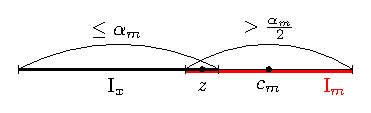
\includegraphics[width=0.45\textwidth]{RAL5_1.eps}
				\caption{Непустое пересечение отрезков $\MI_x$ и $\MI_m$.}
				\label{5_1}
			\end{figure}
			Отсюда, если $5\MI_m$ это отрезок с центром $c_m$, имеющий длину в $5$ раз больше, чем $\MI_m$, то в силу неравенства выше, получим: $\MI_x \subseteq 5\MI_m$;
		\end{enumerate}
		Таким образом, мы получаем:
		$$
			E \setminus \bigsqcup\limits_{n = 1}^{\infty}\MI_{n} \subseteq \bigcup\limits_{m = N+ 1}^{\infty}5\MI_m \Rightarrow \mu^*\left(E \setminus \bigsqcup\limits_{n = 1}^{\infty}\MI_{n}\right) \leq \ddsum{m = N + 1}{\infty}\mu(5\MI_m) = 5 \ddsum{m = N + 1}{\infty}\mu(\MI_m) < \gamma
		$$
		где мы перешли к $\mu$, поскольку все $5\MI_m$ - измеримы. Поскольку $\gamma > 0$ - произвольное, то отсюда вытекает утверждение теоремы. Более того, отсюда вытекает, что множество $E \setminus \bigsqcup\limits_{n = 1}^{\infty}\MI_{n}$ измеримо;
	\end{enumerate}
\end{proof}
\begin{rem}
	Если бы мы использовали $\mu^*$ вместо $\mu$, то возник бы вопрос, почему множество измеримо.
\end{rem}

\begin{corollary}
	В условиях теоремы Витали существует конечный набор попарно непересекающихся отрезков $\{\MI_n\}_{n = 1}^{N} \subset K $ такой, что:
	$$
		\ddsum{n = 1}{N}\mu(\MI_n) > \dfrac{\mu^*(E)}{2}
	$$
\end{corollary}
\begin{rem}
	Если счётным набором отрезков мы можем покрыть всё множество $E$, то выбирая какой-то конечный набор мы можем добиться, чтобы его мера была велика.
\end{rem}

\begin{theorem}
	Пусть $G$ это открытое множество в $\MR^1$, тогда будет верно представление: 
	$$
		G = \bigsqcup\limits_{n = 1}^{\infty}(\alpha_n, \beta_n)
	$$ 
	где один или два интервала могут иметь бесконечные концы.
\end{theorem}
\begin{proof}
	Введём на $G$ отношение эквивалентности: $x \sim y\Leftrightarrow \exists \, (a,b) \in G \colon x,y \in (a,b)$, проверим это:
	\begin{enumerate}[label=\arabic*)]
		\item $G$ - открыто $\Rightarrow \exists \, (a,b) \colon x \in (a,b)$;
		\item Симметричность очевидна;
		\item Пусть $x \sim y, \, y \sim z \Rightarrow \exists \, (a,b), (c,d) \in G \colon x,y \in (a,b), \, y,z \in (c,d) \Rightarrow (a,b)\cap (c,d) \neq \VN$, тогда:
		$$
			(a,b) \cup (c,d) = (\min(a,c), \max(b,d)) = (e,f) \subset G \Rightarrow x,z \in (e,f) \Rightarrow x \sim z
		$$
	\end{enumerate}
	Поэтому всё $G$ представится в виде: $G = \bigsqcup\limits_{\alpha \in A}K_\alpha$, где $K_\alpha$ - класс эквивалентности $\alpha$. Введём обозначение:
	$$
		\forall \alpha, \, a_\alpha = \inf\{x \in K_\alpha\}, \, b_\alpha = \sup\{x \in K_\alpha\}
	$$
	и проверим, что $K_\alpha = (a_\alpha, b_\alpha)$. Действительно, если $x \in (a_\alpha,b_\alpha)$, то:
	$$
		\exists \, y,z \in (a_\alpha,b_\alpha) \cap K_\alpha \colon y \sim z \wedge y < x < z \Rightarrow x \sim y \Rightarrow x \in K_\alpha
	$$
	Если $x \in (-\infty,a_\alpha) \cup (b_\alpha, + \infty)$, то $x\not\in K_\alpha$ по определению $a_\alpha, b_\alpha$. Проверим, что $a_\alpha \not\in K_\alpha$, где $a \neq -\infty$. Для $b_\alpha$ - аналогично. Пусть $a_\alpha \in K_\alpha$, тогда рассмотрим точку $l = a_\alpha + \VE$, где $\VE < (b_\alpha - a_\alpha)$. По предположению верно: $a_\alpha \sim l$, следовательно $\exists \, (\gamma,\delta) \subset G \colon a_\alpha, l \in (\gamma,\delta) \Rightarrow \gamma < a_\alpha$ и кроме того, если мы рассмотрим середину отрезка $(\gamma,a_\alpha) \colon q = \tfrac{a_\alpha + \gamma}{2}$, то:
	$$
		q = \dfrac{a_\alpha +  \gamma}{2} \in (\gamma,\delta) \wedge q < a_\alpha \Rightarrow q \sim a_\alpha \Rightarrow q \in K_\alpha
	$$
	Следовательно, мы получили противоречие с тем, что $a_\alpha$ было точной нижней гранью по всем $x \in K_\alpha$ и $q < a_\alpha \Rightarrow a_\alpha \not\in K_\alpha$. Так как в любом интервале есть рациональное число, то число классов $K_\alpha$ не более, чем счётно. 
\end{proof}

\end{document}